\newpage

\section{Resoconto delle attività di verifica} \label{ResocontoAttivitaVerifica}
In questa sezione viene riportata una sintesi conclusiva dei risultati ottenuti dalle fasi di verifica effettuate nei vari periodi del progetto attraverso le metriche indicate in tale documento. Essi possono coincidere o meno con i valori desiderati da AlphaSix e, nel secondo caso in particolar modo, saranno oggetto di valutazioni per il miglioramento descritte all'appendice \S\ref{mitigazione variazioni}.

I test che vengono introdotti nel corso del progetto non vanno a sostituire i test precedentemente sviluppati. Ogni test, appena è creato viene eseguito periodicamente fino alla fine del progetto, per evitare che i nuovi cambiamenti possano reintrodurre errori precedentemente risolti.

	\subsection{Classificazione dei risultati} \label{classificazionerisultati}
	I risultati ottenuti tramite una metrica, rispetto all'obiettivo che vogliamo raggiungere e ai valori da noi desiderati, sono classificati in:
    
    \begin{itemize}
    	\item \textbf{Soddisfacente}: il risultato è quello atteso.
    	\item \textbf{Poco soddisfacente}: il risultato non è quello atteso, ma gli è vicino.
    	\item \textbf{Insoddisfacente}: il risultato non è per niente quello atteso.
    \end{itemize} 

	\subsection{Primo periodo (RR)}\label{ResocontoAttivitaVerifica:RP}
	Periodo individuato come \AdR\ che dura circa un mese di tempo e un quarto del tempo complessivo per realizzare il progetto.

    \subsubsection{Riassunto delle attività di verifica}
    L'attività di verifica si è rivelata per noi più faticosa del previsto. I motivi sono molteplici:
    	\begin{itemize}
    		\item Nel primo periodo perché non avevamo sufficiente esperienza per effettuare una verifica sistematica e perché la nostra attenzione si è interamente concentrata sull'organizzazione dei ruoli e la loro funzione
    		\item Nel secondo periodo invece la verifica è stata più sistematica e meno impegnativa perché gli elaborati venivano consegnati in orario, ma comunque la correzione si è rivelata onerosa
    	\end{itemize}
    

    Come indicato nelle \NdPd, l'attività di verifica è stata effettuata inizialmente attraverso Walkthrought e successivamente attraverso Inspection. Essendo ancora alle prime armi all'inizio del progetto, abbiamo effettuato la verifica secondo Walkthrough per una buona parte del periodo di analisi dei requisiti realizzata insieme. Dopodiché siamo passati ad adottare Inspection in quanto una ricerca dispersiva non era utile alla parallelizzazione dei compiti. 
    Nel momento in cui sarà necessario verificare prodotti software, riteniamo opportuno effettuare il passaggio da Walkthrough a Inspection in tempi più rapidi rispetto a come è avvenuto finora.
    
    \subsubsection{Risultati delle verifiche tramite analisi}
    Nelle tabelle seguenti vengono riportati i risultati ottenuti applicando le metriche in correlazione all'obiettivo scelto. 
    In ogni tabella sono indicati i prodotti o i processi sottoposti alle metriche e i risultati ottenuti sono presenti in ``Valutazione'', classificati secondo \S\ref{classificazionerisultati}.

    \paragraph{Documenti}

    \begin{table}[H]
    	{\def\arraystretch{1.5}
   		\begin{tabularx}{\textwidth}{YYY}
   			\rowcolor{white}
   			\textbf{QPD001 Leggibilità del testo} & \textbf{MPD001 Indice Gulpease} & \textbf{50 - 60} \\
			\hline
   			\rowcolor{gray!30}
   			\textbf{Prodotto/processo testato} & \textbf{Risultato ottenuto} & \textbf{Valutazione} \\
   			\toprule
   			\rowcolor{white} 	\NdPd & 54.57 & Soddisfacente \\
   			\rowcolor{\grigiodesc} 		\SdFd & 53.7 & Soddisfacente \\
   			\rowcolor{white} 	\PdPd & 51.75 & Soddisfacente \\
   			\rowcolor{\grigiodesc} 	\PdQd & 53.29 & Soddisfacente \\
   			\rowcolor{white} \AdRd & 55.62 & Soddisfacente \\
   			\toprule %\rowcolor{gray!30}
   			\multicolumn{3}{>{\hsize=\dimexpr3\hsize+4\tabcolsep}Y}{\textbf{Nota}: tutti i documenti soddisfano pienamente l'obiettivo di qualifica indicato.} \\ 
   		\end{tabularx}}
   	\caption{Risultati di MPD001 Indice Gulpease}
    \end{table}

	\mydoublerule{\linewidth}{0pt}{2pt}

	\begin{table}[H]
		{\def\arraystretch{1.5}
		\begin{tabularx}{\textwidth}{YYY}
			\rowcolor{white}
			\textbf{QPD002 Correttezza ortografica} & \textbf{MPD002 Correttezza
				ortografica} & \textbf{0} \\
			\hline
			\rowcolor{gray!30}
			\textbf{Prodotto/processo testato} & \textbf{Risultato ottenuto} & \textbf{Valutazione} \\
			\toprule
			\rowcolor{white} \NdPd & 0 & Soddisfacente \\
			\rowcolor{\grigiodesc} \SdFd & 0 & Soddisfacente \\
			\rowcolor{white} \PdPd & 0 & Soddisfacente \\
			\rowcolor{\grigiodesc} \PdQd & 0 & Soddisfacente \\
			\rowcolor{white} \AdRd & 0 & Soddisfacente \\
			\bottomrule
			\multicolumn{3}{>{\hsize=\dimexpr3\hsize+4\tabcolsep}Y}{\textbf{Nota}: tutti i documenti soddisfano pienamente l'obiettivo di qualifica indicato.} \\
		\end{tabularx}}
	\caption{Risultati di MPD002 Correttezza
		ortografica}
	\end{table}

	\paragraph{Processi}

		
		\begin{table}[H]
			{\def\arraystretch{1.5}
				\begin{tabularx}{\textwidth}{YYY}
					\rowcolor{white}
					\textbf{QPR001 Rispetto dei periodi della pianificazione} & \textbf{MPR001 Varianza della pianificazione} & \textbf{96 ore} \\
					\hline
					\rowcolor{gray!30}
					\textbf{Prodotto/processo testato} & \textbf{Risultato ottenuto} & \textbf{Valutazione} \\
					\toprule
					\rowcolor{white} \PdP & 7 & Soddisfacente \\
					\toprule
					\multicolumn{3}{>{\hsize=\dimexpr3\hsize+4\tabcolsep}Y}{\textbf{Nota}: non tutte le scadenze sono state rispettate, ma i ritardi sono rientrati nei valori tollerati. Il valore ottenuto è la somma delle ore di variazione dei vari ruoli.} \\
			\end{tabularx}}
			\caption{Risultati di MPR001 Varianza della pianificazione}
		\end{table}
	
		% \vspace{5pt}
		\mydoublerule{\linewidth}{0pt}{2pt}
		\vspace{20pt}
	
		\begin{table}[H]
			{\def\arraystretch{1.5}
				\begin{tabularx}{\textwidth}{YYY}
					\rowcolor{white}
					\textbf{QPR002 Variazione del budget} & \textbf{MPR002 Varianza dei costi} & \textbf{\EUR{0 - 200}} \\
					\hline
					\rowcolor{gray!30}
					\textbf{Prodotto/processo testato} & \textbf{Risultato ottenuto} & \textbf{Valutazione} \\
					\toprule\rowcolor{white}
					Differenza consuntivo rimanente e consuntivo di periodo & \EUR{ - 15,00} & Soddisfacente \\ 
					\bottomrule
					\multicolumn{3}{>{\hsize=\dimexpr3\hsize+4\tabcolsep}Y}{\textbf{Nota}: il valore desiderato indicato precedentemente sembra essere fin troppo permissivo. Il dettaglio del risultato ottenuto è indicato nel consuntivo di periodo.} \\
			\end{tabularx}}
			\caption{Risultati di MPR002 Varianza dei costi}
		\end{table}
	
		\mydoublerule{\linewidth}{0pt}{2pt}
		\vspace{20pt}
	
		\begin{table}[H]
			{\def\arraystretch{1.5}
				\begin{tabularx}{\textwidth}{YYY}
					\rowcolor{white}
					\textbf{QPR003 Rispetto delle fasi del ciclo di vita} & \textbf{MPR003 Aderenza agli standard} & \textbf{Livello di maturità: 3 Valutazione attributi: L} \\
					\hline
					\rowcolor{gray!30}
					\textbf{Prodotto/processo testato} & \textbf{Risultato ottenuto} & \textbf{Valutazione} \\
					\toprule\rowcolor{white}
					PROC001 Pianificazione del progetto, organizzazione e struttura & Livello di maturità: 2 Valutazione attributi: L & Poco soddisfacente \\
					\bottomrule
					\multicolumn{3}{>{\hsize=\dimexpr3\hsize+4\tabcolsep}Y}{\textbf{Nota}: essendo il primo periodo è prevedibile che il livello di maturità desiderato non sia ancora quello sperato. Si prevede un miglioramento per le successive revisioni.} \\
			\end{tabularx}}
			\caption{Risultati di MPR003 Aderenza agli standard}
		\end{table}
	
		%\mydoublerule{\linewidth}{0pt}{2pt}
		\vspace{20pt}
		
		\begin{table}[H]
			{\def\arraystretch{1.5}
				\begin{tabularx}{\textwidth}{YYY}
					\rowcolor{white}
					\textbf{QPR004 Versionamento} & \textbf{MPR004 Frequenza commit nella repository} & \textbf{25} \\
					\hline
					\rowcolor{gray!30}
					\textbf{Prodotto/processo testato} & \textbf{Risultato ottenuto} & \textbf{Valutazione} \\
					\toprule\rowcolor{white}
					Repository & 31.25 & Soddisfacente \\
					\bottomrule
					\multicolumn{3}{>{\hsize=\dimexpr3\hsize+4\tabcolsep}Y}{\textbf{Nota}: il numero di commit effettuati risulta ottimo.} \\
			\end{tabularx}}
			\caption{Risultati di MPR004 Frequenza commit nella repository}
		\end{table}
		
		\mydoublerule{\linewidth}{0pt}{2pt}
		\vspace{20pt}
		
		\begin{table}[H]
			{\def\arraystretch{1.5}
				\begin{tabularx}{\textwidth}{YYY}
					\rowcolor{white}
					\textbf{QPR009 Effettuare una verifica costante} & \textbf{MPR009 Frequenza controllo prodotti} & \textbf{5 Modifiche} \\
					\hline
					\rowcolor{gray!30}
					\textbf{Prodotto/processo testato} & \textbf{Risultato ottenuto} & \textbf{Valutazione} \\
					\toprule\rowcolor{white}
					Documenti & 7.2 & Poco soddisfacente \\
					\bottomrule
					\multicolumn{3}{>{\hsize=\dimexpr3\hsize+4\tabcolsep}Y}{\textbf{Nota}: il valore ottenuto non soddisfa il risultato atteso perché nella prima parte del macro periodo \gruppo\ ha prestato molta attenzione alla formazione personale a discapito del tempo che poteva essere dedicato alla verifica dei prodotti.} \\
			\end{tabularx}}
			\caption{Risultati di MPR009 Frequenza controllo prodotti}
		\end{table}
	
	%\mydoublerule{\linewidth}{0pt}{2pt}
	
	\subsection{Secondo periodo (RP)}
	Periodo individuato come Revisione Progettuale la quale dura all'incirca un mese ed un quarto dell'intera durata del progetto.
	
	\subsubsection{Riassunto delle attività di verifica}
	In questo periodo di tempo abbiamo per lo più attuato verifiche sui documenti, come per il periodo di \RR, ma in maniera più approfondita e  sistematica, e verifiche sul software, in particolare sul codice scritto per il \gloss{Proof of Concept}.

	
	\subsubsection{Risultati delle verifiche tramite analisi}
	In questa sezione riportiamo i diagrammi contenenti tutti i valori di nostro interesse per dare un giudizio sul lavoro svolto fino alla fine di questo periodo.
	Essi contengono i valori ottenuti nel tempo partendo dall'ultima consegna dei documenti (il 2019-01-14) e mostrano con chiarezza l'andamento delle misurazioni che abbiamo effettuato.
	Per questo motivo, ogni diagramma è intitolato con la metrica utilizzata ed è accompagnato da:
	\begin{itemize}
		\item \textbf{Obiettivo}: codice dell'obiettivo di qualità.
		\item \textbf{Valore desiderato}: il valore desiderato ottenibile da una determinata metrica.
		\item \textbf{Descrizione}: breve descrizione del diagramma.
		\item \textbf{Valutazione}: la nostra valutazione classificata secondo \S\ref{classificazionerisultati}.
		\item \textbf{Considerazioni}: nostro commento in relazione ai risultati ottenuti dalla misurazione.
	\end{itemize}


	\paragraph{Documenti}

	\subparagraph{MPD001 Indice di Gulpease}

	\begin{figure}[H]
		\centering
		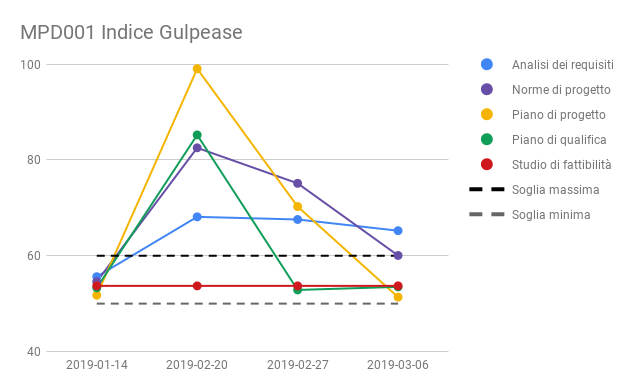
\includegraphics[width=0.9\textwidth]{img/cruscotti/MPD001.png}
		\label{immaginegulpease}
		\caption{Diagramma con valori misurati tramite MPD001 Indice di Gulpease}
	\end{figure}

	\begin{itemize}
		\item \textbf{Obiettivo}: QPD001 Leggibilità del testo.
		\item \textbf{Valore desiderato}: 50 - 60.
		\item \textbf{Descrizione}: vengono mostrati i cambiamenti dei valori dell'Indice di Gulpease nei documenti e la soglia minima e massima (in grigio e nero) in cui devono rientrare i valori dei documenti. 
		\item \textbf{Valutazione}: soddisfacente.
		\item \textbf{Considerazioni}: ogni documento ha degli alti e bassi nel corso della stesura, ma infine tutti, eccetto l'\AdR, rispettano i valori desiderati.
	\end{itemize}


	\subparagraph{MPD002 Correttezza ortografica}

	\begin{figure}[H]
		\centering
		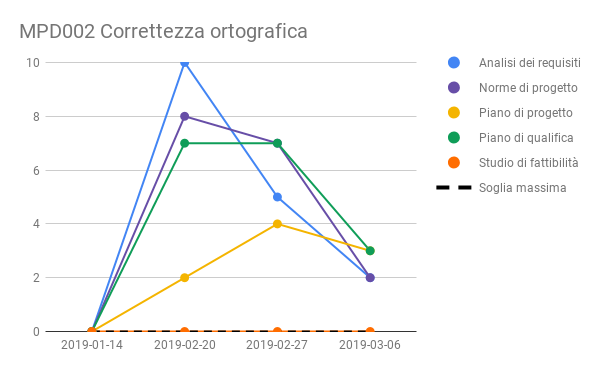
\includegraphics[width=0.9\textwidth]{img/cruscotti/MPD002.png}
		\label{immagineCorrettezzaOrtografica}
		\caption{Diagramma con valori misurati tramite MPD002 Correttezza ortografica}
	\end{figure}

	\begin{itemize}
		\item \textbf{Obiettivo}: QPD002 Correttezza ortografica.
		\item \textbf{Valore desiderato}: 0.
		\item \textbf{Descrizione}: per ogni documento è mostrato l'andamento del numero di errori ortografici e la soglia (in nero) messa a zero.
		\item \textbf{Valutazione}: soddisfacente.
		\item \textbf{Considerazioni}: dopo la modifica iniziale dei documenti il numero di errori è diminuito, tendendo ad annullarsi per la fine del periodo \RP.
	\end{itemize}



	\paragraph{Processi}

	\subparagraph{MPR001 Varianza della pianificazione}

	\begin{figure}[H]
		\centering
		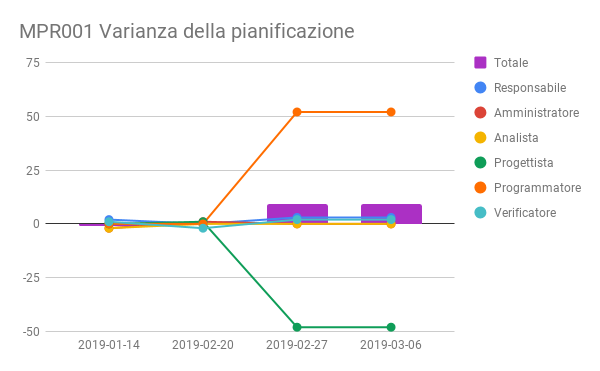
\includegraphics[width=0.9\textwidth]{img/cruscotti/MPR001.png}
		\label{immagineVarianzaPianificazione}
		\caption{Diagramma con valori misurati tramite MPR001 Varianza della pianificazione}
	\end{figure}

	\begin{itemize}
		\item \textbf{Obiettivo}: QPR001 Rispetto dei periodi della pianificazione.
		\item \textbf{Valore desiderato}: 96 ore.
		\item \textbf{Descrizione}: oltre a mostrare le ore di varianza di ogni ruolo, viene mostrato anche il totale delle ore di variazione (in viola) coi relativi valori. 
		\item \textbf{Valutazione}: poco soddisfacente.
		\item \textbf{Considerazioni}:Nelle ultime settimane siamo stati costretti a ridurre drasticamente le ore al \Prog\ per darne al \Progr\ essendo a ridosso della consegna del Proof of Concept. Questo purtroppo ha portato ad una variazione troppo elevata del preventivo in termini di ore.
	\end{itemize}


	\subparagraph{MPR002 Varianza dei costi}

	\begin{figure}[H]
		\centering
		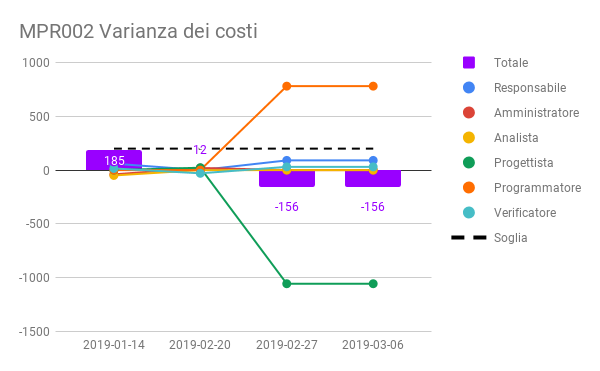
\includegraphics[width=0.9\textwidth]{img/cruscotti/MPR002.png}
		\label{immagineVarianzaCosti}
		\caption{Diagramma con valori misurati tramite MPR002 Varianza dei costi}
	\end{figure}

	\begin{itemize}
		\item \textbf{Obiettivo}: QPR002 Varianza del budget.
		\item \textbf{Valore desiderato}: \EUR{0 - 200}.
		\item \textbf{Descrizione}: vengono mostrate le variazioni della spesa attribuita ad ogni ruolo, inoltre ne viene mostrato il totale attraverso delle colonne (in viola) coi relativi valori.
		\item \textbf{Valutazione}: soddisfacente.
		\item \textbf{Considerazioni}: la diminuzione delle ore assegnate al \Prog\ a favore di quelle per il \Progr, ha portato ad una diminuzione di \EUR{156} del preventivo, un dato che comunque risulta essere soddisfacente.
	\end{itemize}
	

	\subparagraph{MPR003 Aderenza agli standard}

	\begin{figure}[H]
		\centering
		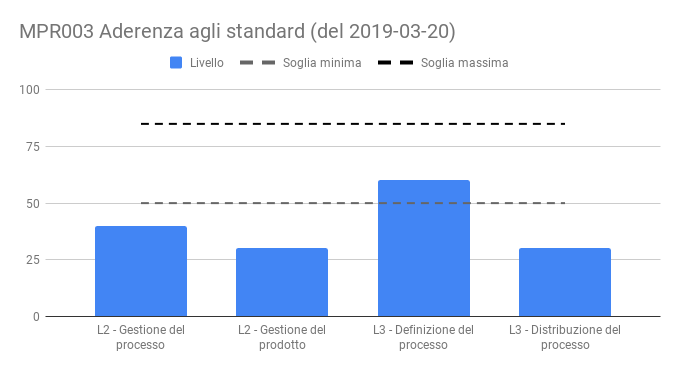
\includegraphics[width=0.9\textwidth]{img/cruscotti/MPR003_(1).png}
		\label{immagineAderenzaStandard1}
		\caption{Diagramma con valori misurati tramite MPR003 Aderenza agli standard (1)}
	\end{figure}

    \begin{figure}[H]
        \centering
        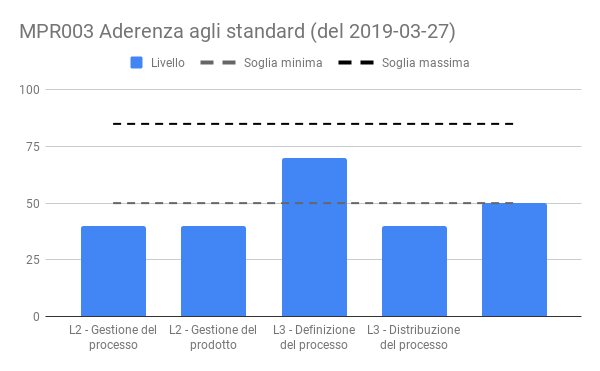
\includegraphics[width=0.9\textwidth]{img/cruscotti/MPR003_(2).png}
        \label{immagineAderenzaStandard2}
        \caption{Diagramma con valori misurati tramite MPR003 Aderenza agli standard (2)}
    \end{figure}
    
    \begin{figure}[H]
        \centering
        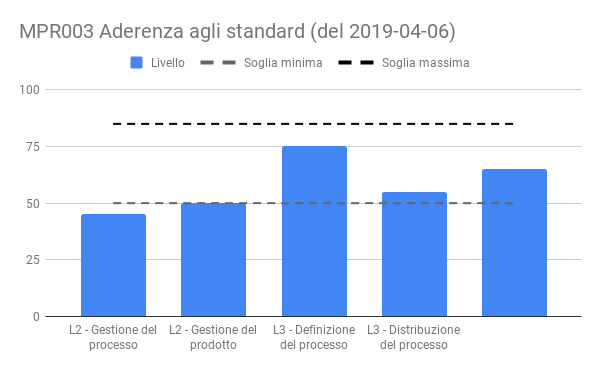
\includegraphics[width=0.9\textwidth]{img/cruscotti/MPR003_(3).png}
        \label{immagineAderenzaStandard3}
        \caption{Diagramma con valori misurati tramite MPR003 Aderenza agli standard (3)}
    \end{figure}

	\begin{itemize}
		\item \textbf{Obiettivo}: QPR003 Rispetto delle fasi del ciclo di vita.
		\item \textbf{Valore desiderato}: Livello di maturità: 3, Valutazione attributi: L.
		\item \textbf{Descrizione}: per ogni attributo dei processi viene mostrato in che percentuale sono soddisfatti attraverso le colonne (in blu), mostrando anche la soglia minima e massima (in grigio e nero) che questi valori dovrebbero avere.
		\item \textbf{Valutazione}: poco soddisfacente.
		\item \textbf{Considerazioni}: il miglioramento per quanto riguarda l'aderenza agli standard è presente, ma non ancora sufficiente per gli obiettivi prefissati.
	\end{itemize}
	



	\paragraph{Software}

	\subparagraph{MPS001 Presenza di bug}
    
    \begin{figure}[H]
        \centering
        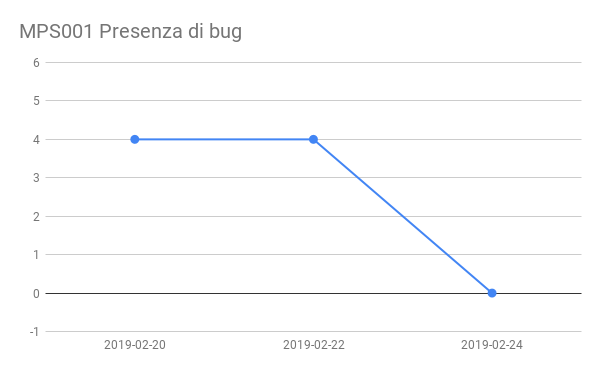
\includegraphics[width=0.9\textwidth]{img/cruscotti/MPS001.png}
        \label{immaginePresenzaBug}
        \caption{Diagramma con valori misurati tramite MPS001 Presenza di bug}
    \end{figure}
    
    \begin{itemize}
        \item \textbf{Obiettivo}: QPS001 Assenza di bug.
        \item \textbf{Valore desiderato}: 0.
        \item \textbf{Descrizione}: viene mostrato il numero totale di bug rilevati da SonarQube.
        \item \textbf{Valutazione}: soddisfacente.
        \item \textbf{Considerazioni}: per la consegna del Proof of Concept abbiamo cercato di togliere tutti i bug presenti nel codice.
    \end{itemize}

    \subparagraph{MPS002 Presenza di vulnerabilità}
    
    \begin{figure}[H]
        \centering
        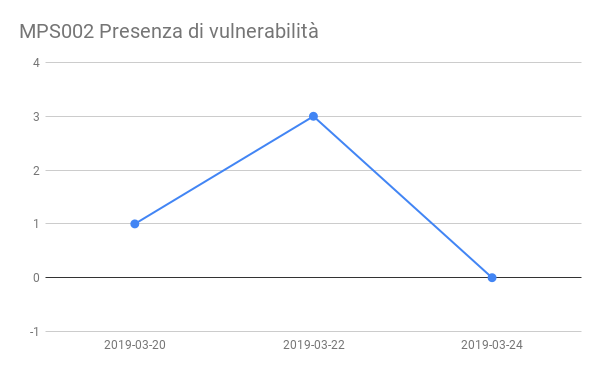
\includegraphics[width=0.9\textwidth]{img/cruscotti/MPS002.png}
        \label{immaginePresenzaVulnerabilità}
        \caption{Diagramma con valori misurati tramite MPS002 Presenza di vulnerabilità}
    \end{figure}
    
    \begin{itemize}
        \item \textbf{Obiettivo}: QPS002 Assenza di vulnerabilità.
        \item \textbf{Valore desiderato}: 0.
        \item \textbf{Descrizione}: viene mostrato il numero totale di vulnerabilità rilevate da SonarQube.
        \item \textbf{Valutazione}: soddisfacente.
        \item \textbf{Considerazioni}: per la consegna del Proof of Concept abbiamo cercato di togliere tutte le vulnerabilità presenti nel codice.
    \end{itemize}

    \subparagraph{MPS003 Presenza di code smell}
    
    \begin{figure}[H]
        \centering
        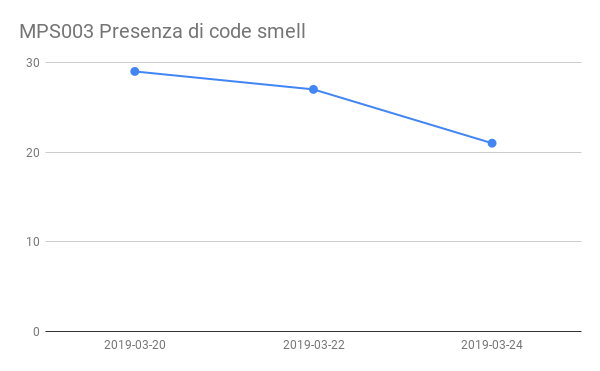
\includegraphics[width=0.9\textwidth]{img/cruscotti/MPS003.png}
        \label{immaginePresenzaCodeSmell}
        \caption{Diagramma con valori misurati tramite MPS003 Presenza di code smell}
    \end{figure}
    
    \begin{itemize}
        \item \textbf{Obiettivo}: QPS003 Assenza di code smell.
        \item \textbf{Valore desiderato}: 0.
        \item \textbf{Descrizione}: viene mostrato il numero totale di code smell rilevati da SonarQube.
        \item \textbf{Valutazione}: poco soddisfacente.
        \item \textbf{Considerazioni}: dato che non risultano essere errori particolarmente gravi all'interno del codice si ha dato priorità a correggere altri tipi di errori prima della consegna del Proof of Concept. Prevediamo di toglierli completamente nelle parti utilizzeremo successivamente per il prodotto finale.
    \end{itemize}

    \subparagraph{MPS004 Duplicazione del codice}
    
    \begin{figure}[H]
        \centering
        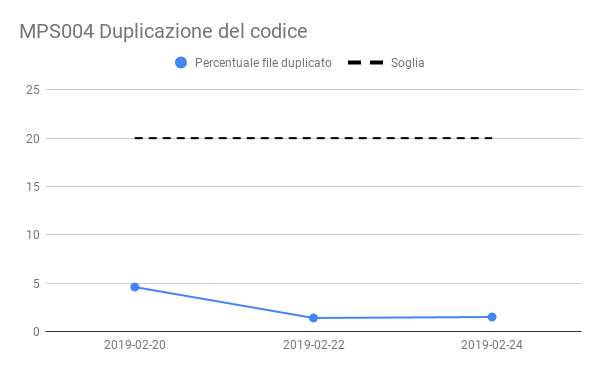
\includegraphics[width=0.9\textwidth]{img/cruscotti/MPS004.png}
        \label{immaginePresenzaDupplicazioneCodice}
        \caption{Diagramma con valori misurati tramite MPS004 Duplicazione del codice}
    \end{figure}
    
    \begin{itemize}
        \item \textbf{Obiettivo}: QPS004 Minima duplicazione del codice.
        \item \textbf{Valore desiderato}: 0 - 20\%.
        \item \textbf{Descrizione}: viene mostrata la percentuale di codice duplicato rilevato da SonarQube.
        \item \textbf{Valutazione}: soddisfacente.
        \item \textbf{Considerazioni}: La quantità di codice duplicato, dopo la prima verifica, è rimasto molto basso. Miriamo ad abbassarlo ulteriormente nel prossimo periodo, ma di non raggiungere ad un totale 0\%.
    \end{itemize}